\documentclass{beamer}
%\documentclass[final]{beamer}

\mode<presentation>
{
%  \usetheme{default}
%  \usetheme{boxes}
  \usetheme{Boadilla}
}

\AtBeginSection[] 
{ 
  \begin{frame}[plain]{Outline} 
    \tableofcontents[currentsection,
    subsectionstyle=shaded/shaded/shaded
    ] 
  \end{frame} 
}

\AtBeginSubsection[] 
{ 
  \begin{frame}[plain]{Outline} 
    \tableofcontents[currentsection,currentsubsection] 
  \end{frame} 
}


\usepackage{amsmath, amssymb}
\usepackage{algorithm, algorithmic}
\usepackage{listings}
\lstset{%
language=Python,
backgroundcolor=\color{yellow},
}
\usepackage{multirow}
\usepackage{textpos}
\usepackage{subfigure}

\usepackage{tikz}
\usepackage{pbox}

\DeclareMathOperator{\poly}{poly}
\DeclareMathOperator{\nnz}{nnz}
\DeclareMathOperator{\bigO}{\mathcal{O}}

\renewcommand{\thefootnote}{\fnsymbol{footnote}}

\renewcommand{\algorithmicrequire}{\textbf{Input:}}
\renewcommand{\algorithmicensure}{\textbf{Output:}}

\newtheorem{assumption}{Assumption}
\newtheorem{condition}{Condition}

\newcommand{\icon}[2][1]{\begingroup
\setbox0=\hbox{\includegraphics[scale=#1,keepaspectratio]{#2}}%
\parbox{\wd0}{\box0}\endgroup}

\newcommand{\Diagnl}[1]{\mbox{}{Diag}\left\{#1\right\}}
\newcommand{\Expect}[1]{\mbox{}{\mathbb{E}}\left[#1\right]}
\newcommand{\ExpectSub}[2]{\mbox{}{\mathbb{E}}_{#1}\left[#2\right]}
%\newcommand{\Expect}[1]{\mbox{}{\bf{E}}\left[#1\right]}
\newcommand{\CExpect}[1]{\mbox{}{\bf{E}_{w}}\left[#1\right]}
\newcommand{\Varnce}[1]{\mbox{}{\bf{Var}}\left[#1\right]}
\newcommand{\CVarnce}[1]{\mbox{}{\bf{Var}_{w}}\left[#1\right]}

%\renewcommand{\thefootnote}{\fnsymbol{footnote}}
%
%\renewcommand{\algorithmicrequire}{\textbf{Input:}}
%\renewcommand{\algorithmicensure}{\textbf{Output:}}

% From Miles
\newcommand{\R}{\mathbb{R}}
\newcommand{\argmin}{\text{argmin}}
\newcommand{\ts}{\textstyle}
\newcommand{\ttop}{^{\top}}
%\usepackage{color}
\definecolor{darkgreen}{rgb}{0.0, 0.4, 0.0}
\newcommand{\opt}{\textup{opt}}
\newcommand{\ve}{\varepsilon}

% From Xinlian
\newcommand{\sbf}{\boldsymbol}
\newcommand{\mbf}{\mathbf}

\usepackage{makecell}

\usepackage[T1]{fontenc}
\usepackage[utf8]{inputenc}
\usepackage{lmodern,tabularx,ragged2e}
\newcolumntype{Y}{>{\arraybackslash\RaggedRight}X}
\newcolumntype{P}[1]{>{\arraybackslash\RaggedRight}p{#1}}

%\usepackage[all]{xy}

%\usepackage{enumitem}

\usepackage[normalem]{ulem}

\begin{document}

\title[Practical Theory \& NN Models]{ Practical Theory and Neural Network Models }

\begin{frame}
  \frametitle{Exact expressions for double descent and\\
implicit regularization\hfill 
\footnotesize{\it with Micha{\l } Derezi\'{n}ski and  Feynman Liang}}

\begin{columns}
  \begin{column}{0.5\textwidth}
    \begin{center}
      {
        \large\underline{Double descent}}
    \end{center}
    \vspace{2mm}
    \small
    
    ``Classical'' ML: \hfill\textit{parameters} $\ll$ \textit{data}\quad~\\
    ``Modern'' ML: \hfill \textit{parameters} $\gg$ \textit{data}\quad~\\
\textit{Phase transition:} \hfill\textit{parameters} $\sim$ \textit{data}\quad~\\[7mm]
\textbf{Our contribution:}\\
New \textit{exact} analysis for a linear model
    
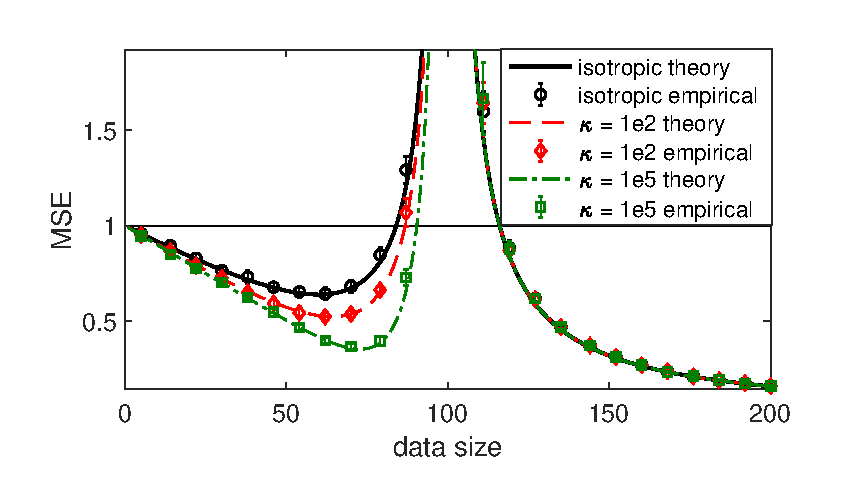
\includegraphics[width=\textwidth]{figs/descent-intro-nice}
\vspace{2mm}

{\footnotesize
%  Belkin, Hsu, Ma, Mandal (2019). arXiv:1812.11118\\
\mbox{Hastie, Montanari, Rosset, Tibshirani (2019).~arXiv:1903.08560}\\
   Bartlett, Long, Lugosi, Tsigler (2019). arXiv:1906.11300\\
}
  

\end{column}
\begin{column}{0.5\textwidth}
    \begin{center}
      {
        \large\underline{Implicit regularization}}
  \end{center}
  \vspace{2mm}
  \small
  
Why does ``Modern'' ML work?\\
Because it induces implicit regularization\\[11mm]
\textbf{Our contribution:}\\
Implicit \textit{ridge} regularization of the\\
minimum-norm solution $\mathbf{X}^\dagger\mathbf{y}$
\vspace{3mm}
  \begin{align*}
    \hspace{-2mm}\mathbb{E}[\mathbf{X}^\dagger\mathbf{y}]
    &\simeq
      \argmin_{\mathbf{w}}\mathbb{E}\big[(\mathbf{x}^\top\mathbf{w}-y)^2\big] + \overbrace{\lambda
    \,\|\mathbf{w}\|^2}^{\text{ridge}}\\
&\quad\text{when parameters $\gg$ data}
  \end{align*}
  \vspace{7mm}

  {\footnotesize
    Mahoney (2012). arXiv:1203.0786\\
    Neyshabur, Tomioka, Srebro (2014). arXiv:1412.6614\\
    }
\end{column}
\end{columns}
 
\end{frame}

\end{document}


